\documentclass[11pt,letterpaper]{article}
\usepackage[utf8]{inputenc}
\usepackage[spanish,USenglish]{babel}
\usepackage{amsmath}
\usepackage{amsfonts}
\usepackage{amssymb}
\usepackage{amsthm}
\usepackage{graphicx}
\usepackage[left=2cm,right=2cm,top=2cm,bottom=2cm]{geometry}
\usepackage{flushend}
\usepackage{pgf,tikz, pgfplots}
\usetikzlibrary{arrows}
\pgfplotsset{compat=1.15}
\usepackage{pgf,tikz,pgfplots}
%escribir programas
\usepackage{listings}
\usepackage{algpseudocode}
\usepackage{algorithm}
\renewcommand{\algorithmicrequire}{\textbf{Input:}}
\renewcommand{\algorithmicensure}{\textbf{Output:}}

%encabezado
\usepackage{fancyhdr}
\pagestyle{fancy}
\fancyhf{}
\fancyhead[RO]{\thepage} % Números de página en las esquinas de los encabezados
%%%%%%%%%%%%%%%%%%%% BOXES %%%%%%%%%%%%%%%%%%%
\usepackage{bm}
\newcommand{\commentedbox}[2]{%
	\mbox{
		\begin{tabular}[t]{@{}c@{}}
			$\boxed{\displaystyle#1}$\\
			#2
		\end{tabular}%
	}%
}
\usepackage{framed}
\usepackage{wrapfig}\definecolor{shadecolor}{RGB}{224,238,238}
%%%%%%%%%%%%%%%%%%%%%%%%% DEFINITIONS %%%%%%%%%%%%%%%%%%%%%%%%
\theoremstyle{definition}
\newtheorem{defi}{Definición}[section]%Para definiciones
\theoremstyle{definition}
\newtheorem{teo}{Teorema}[section]%Para definiciones
\newtheorem{prop}{Proposición}
\theoremstyle{definition}
\newtheorem{ej}{Ejemplo}[section]
\newtheorem{lem}{Lema}
\newtheorem{prblm}{Problema}
\newtheorem{col}{Corolario}[section]



\title{\textbf{Tarea 4: Steepest Descent}\\ Optimización I \\ \Large {Maestría en Computación}\\ \Large {Centro de Investigación en Matemáticas}}
\author{Esteban Reyes Saldaña \\ esteban.reyes@citmat.mx}

\begin{document}

\selectlanguage{spanish}
\twocolumn[
\begin{@twocolumnfalse}
	\maketitle
	\begin{center}\rule{0.9\textwidth}{0.1mm} \end{center}
	\begin{abstract}
		\normalsize{En esta tarea se implementó el método de descenso gradiente usando búsqueda en línea con backtracking y el método de bisección. Se presenta a continuación una descripción general del método, así como el pseudocódigo de los mpetodos implementados. En los resultados se incluyen pruebas para diferentes funciones tanto como para los puntos iniciales sugeridos por el Profesor como puntos iniciales aleatorios. Finalmente se incluyen algunas conclusiones observadas a partir de la experimentación.}
	\begin{center}\rule{0.9\textwidth}{0.1mm} \end{center}
	\end{abstract}
\end{@twocolumnfalse}]

\section{Introducción}

El objetivo general es encontrar los mínimos locales de una función $ f : \mathbb{R}^n \to \mathbb{R} $ tal que $ f(x) \in\mathcal{C}^1 $ de manera iterativa. El algoritmo general se ve como
\begin{shaded*}
\begin{enumerate}
	\item Eliga un punto inicial $ x_0 $ y haga $ k = 0 $.
	\item Mientras no converja
		\begin{enumerate}
			\item Encuentre $ x_{k+1} $ tal que $ f(x_{k+1}) < f(x_k) $
			\item $ k \to k + 1 $		
		\end{enumerate}
	\item Regrese $ x^* = x_k $.
\end{enumerate}
\end{shaded*}

\begin{shaded*}
\begin{defi}
	Sea $ f: \mathbb{R}^n \to \mathbb{R} $ una función continuamente diferenciable. El gradiente de $ f $ en el punto $ p $ está dado por
	\[ \nabla^T f(p) = \left[ \dfrac{\partial f(p)}{\partial x_1}, \dfrac{\partial f(p)}{\partial x_2}, \dots, \dfrac{\partial f(p)}{\partial x_n} \right] \]
\end{defi}
\end{shaded*}
En clase se vieron algunos resultados sobre el gradiente.

\begin{shaded*}
\begin{teo}
	Sea $ f: \mathbb{R}^n \to \mathbb{R} $ una función continuamente diferenciable. Entonces para toda $ x  \in dom(f) $, $ \nabla f(x) $ es perpendicular al conjunto de nivel
	\[ S = \{ x \in \mathbb{R}^n | f(x) = c, c\textup{ constante.} \} \]
\end{teo}
\end{shaded*}

\begin{shaded*}
\begin{teo}\label{max_}
	Sea $ f: \mathbb{R}^n \to \mathbb{R} $ una función continuamente diferenciable. Entonces la dirección donde $ f(x) $ crece más rápido es $ \nabla f(x) $.
\end{teo}
\end{shaded*}

\begin{col}
	Bajo las condiciones del Teorema (\ref{max_}), $ f(x) $ decrece más rápido en la dirección $ - \nabla f(x) $.
\end{col}

Sin embargo, existen algoritmos no monótonos en los que $ f(x) $ no decrece en cada paso si no después de un número $ m $ de iteraciones, esto es
\[ f(x_{k+1} < f(x_{k-j})) \]
para algún $ j \in \{ 0, 1, \dots, M \} $ con $ M = m-1 $ si $ k\geq m -1 $ y $ M = k $ en otro caso.	
Así que ahora surgen tres preguntas
\begin{enumerate}
	\item ¿Cómo elegir $ x_0 $?
	\item ¿Qué criterio de paro usar?
	\item ¿Cómo actualizar $ x_{k+1} $?
\end{enumerate}	

\begin{shaded*}
\begin{defi}
	Una \textbf{dirección de descenso} $ d \in \mathbb{R}^n $ para $ f \in \mathcal{C}^1 $ es un vector tal que
	\[ f(x + t d) < f(x) \]
	para $ t \in (0, T) $. Es decir, permite que el punto $ x $ más cerca al mínimo local $ x^* $ de la función objetivo $ f: \mathbb{R}^n \to \mathbb{R} $.
\end{defi}
\end{shaded*}

\begin{shaded*}
\begin{teo}
	Si $ g(x)^T d < 0 $ entonces $ d $ es una dirección de descenso.
\end{teo}
\end{shaded*}
\textbf{Observación.} La dirección 
\[ d_k = - g(x_k) \]
es la elección más obvia de una dirección de búsqueda.
\section{Método}
\subsection{Steepest Descent}
Este es un método de búsqueda en línea que usa la dirección $ d_k = - g(x_k) $ para moverse en cada iteración. El esquema general es
\begin{enumerate}
	\item Dé un vector inicial $ x_0 $.
	\item Haga $ k = 0 $ y $ g_0 = \nabla f(x_0) $
	\item Mientras $ || g_k || \neq 0 $, 
			\begin{enumerate}
				\item $ \alpha_k = \displaystyle\arg \min_{\alpha >0} f(x_k - \alpha g_k) $
				\item $ x_{k+1} = x_k - \alpha_k g_k $
				\item $ g_{k+1} = \nabla f (x_{k+1}) $
				\item $ k \to k + 1 $
			\end{enumerate}
\end{enumerate}
Se debe seleccionar un tamaño de paso $ \alpha_k $ tal que reduce suficientemente a $ f(x) $ y al mismo tiempo se requiere que sea eficiente. Para ello se plantea encontrar el tamaño de paso como encontrar una aproximación del problema de optimización previo. La búsqueda en línea se hace en dos pasos iterativos
\begin{shaded*}
	\begin{enumerate}
		\item Una fase donde se acota el intervalo que contiene el tamaño de paso deseado,
		\item una bisección o interpolación que calcula un ''buen´´ tamaño de paso con dicho intervalo.
	\end{enumerate}
\end{shaded*}
\subsection{Condición de Armijo}
Un tamaño de decrecimiento suficiente se puede medir por la siguiente ecuación
\[  f(x_k + \alpha d_k) \leq f(x_k) + c_1 \alpha \nabla f_k^T d_k, \]
para alguna constante $ c_1 \in (0,1) $.
\\
Una condición suficiente de descenso no es suficiente por sí mismoa para asegurar que el algoritmo progresa de manera adecuada ya que se satisiface para valores de $ \alpha $ suficientemente pequeños.
\\
Para obtener pasos más largos, se da una segunda condición, llamada condición de curvatura. 
\subsection{Condiciones de Wolfe}
\begin{eqnarray}
	f(x_k + \alpha d_k) & \leq & f(x_k) + c_1 \alpha \nabla f_k^T d_k, \\
	\nabla f(x_k + \alpha d_k)^T d_k & \geq & c_2 \nabla f_k^T d_k
\end{eqnarray}
con $ 0 < c_1 < c_2 < 1 $. 
\subsection{Pseudocódigo}
\subsubsection{Búsqueda con BackTracking}
\begin{shaded*}
	\begin{algorithmic}[1]
		% ENTRADA / SALIDA
		\Require{$ \hat{\alpha} $, $ \rho \in (0,1) $, $ c_1 \in (0,1) $}
		\Ensure{Tamaño de paso $ \alpha_k $}
		\State{Haga $ alpha = \hat{\alpha} $}
		\State{$inum =0 $}
		\While{$ f(x_k + \alpha d_k) > f(x_k) + c_1 \alpha \nabla f_k^T d_k $}
			\State{$ alpha \to \rho \alpha $}
		\EndWhile
		\State{Regresa $ \alpha_k = \alpha $}
	\end{algorithmic}
\end{shaded*}

\subsubsection{Búsqueda en Línea con Bisección}
\begin{shaded*}
	\begin{algorithmic}[1]
		% ENTRADA / SALIDA
		\Require{$ \alpha_0 $, $ 0 < c_1 < c_2 < 1 $}
		\Ensure{Tamaño de paso $ \alpha_k $}
		\State{Haga $ alpha = 0 $, $ \beta = \infty $, $ \alpha^i = \alpha_0 $}
		\State{$inum =0 $}
		\While{$ f(x_k + \alpha_k d_k) > f(x_k) + c_1 \alpha_k \nabla f_k^T d_k $ \textbf{o} $ \nabla f(x_k + \alpha_k d_k)^T d_k < c_2 \nabla f(x_k)^T d_k $}
			\If{$ f(x_k + \alpha_k d_k) > f(x_k) + c_1 \alpha_k \nabla f_k^T d_k $}
				\State{$ \beta = \alpha_k $}
				\State{$ \alpha_k = \dfrac{\alpha + \beta}{2} $}
			\Else
				\State{$\alpha = \alpha_k $}
				\If{$\beta = \infty $}
					\State{$\alpha_k = 2 \alpha$}
				\Else
					\State{$ \alpha_k = \dfrac{\alpha + \beta}{2} $}
				\EndIf
			\EndIf
		\EndWhile
		\State{Regresa $ \alpha_k $}
	\end{algorithmic}
\end{shaded*}

\subsection{Función de Rosembrock}
\begin{shaded*}
\[ f(x) = \sum_{i = 1}^{N-1} [100(x_{i+1} - x_i^2)^2 + (1 - x_i)^2] \]
donde $ x = [ x_1, \dots, x_N ]^T \in\mathbb{R}^N $.
\end{shaded*}
\textbf{Gradiente}.  Primero notemos que  para $ 2 \leq j \leq N-1 $ se puede reescribir $ f(x) $ como
\begin{eqnarray*}
	f(x) & = & \sum_{i = 1}^{j-2}  [100(x_{i+1}- x_i^2)^2 + (1-x_i)^2] \\
	     &   &  + [100(x_{j} - x_{j-1}^2)^2 + (1-x_{j-1})^2] \\
	&   & [100(x_{j+1} - x_{j}^2)^2 + (1-x_{j})^2] \\
	&   & +  \sum_{i = j+1}^{N-1} [100(x_{i-1} - x_i^2)^2 - (1-x_i)^2 ]. \\
\end{eqnarray*}
Notemos que el primer y útlimo término son constantes con respecto a $ x_j $, entonces se anularán al calcular la correspondiente derivada parcial.
\\
Para $ D_1 $ se tiene que
\begin{eqnarray*}
	\dfrac{\partial }{\partial x_1} f(x) & = & 100(2)(x_2 - x_1^2) (-2x_1) - 2(1-x_1)  \\
	& = &  -400(x_2 - x_1^2)x_1 - 2(1-x_1).
\end{eqnarray*}
Para $ D_j \in\{ 2, \dots, N-1 \} $,
\begin{eqnarray*}
	\dfrac{\partial }{\partial x_j} f(x) & = & [200(x_j - x_{j-1}^2)] + [ 200(x_{j+1} - x_j^2)(-2x_j)] \\
	& & - [2(1-x_j) ] \\
	& = & 200(x_j - x_{j-1}^2) - 400 (x_{j+1} - x_j^2) x_j  \\
	& & - 2(1-x_j)
\end{eqnarray*}
Para $ D_N $, 
\begin{eqnarray*}
	\dfrac{\partial }{\partial x_N} f(x) & = & 200(x_N - x_{N-1}^2).
\end{eqnarray*}
De lo anterior tenemos que
\begin{shaded*}
\footnotesize{
\begin{equation*}
	\nabla f(x)  =  \left[\begin{matrix}
		-400(x_2 - x_1^2) x_1 - 2(1-x_1) \\
		\vdots							 \\
		200(x_j - x_{j-1}^2) - 400(x_{j+1} - x_j^2)x_j - 2(1-x_j)					 \\
		\vdots  						 \\
		200(x_N - x_{N-1}^2).
	\end{matrix}\right]
\end{equation*}}
\end{shaded*}
\textbf{Hessiano}. Para calcular el Hessiano, se debe considerar como casos particulares, aquellos que se apliquen a $ \dfrac{\partial f(x) (x)}{\partial x_1} $ y $ \dfrac{\partial f(x) (x)}{\partial x_N} $ (como se observó en el gradiente). 
\\
Para $ D_{x_k x_1 } $,
\begin{eqnarray*}
	\dfrac{\partial^2 f(x)}{\partial x_k \partial x_1} = \left\{\begin{matrix}
		1200x_1^2 -400 x_2 +2 & si & k = 1 \\
		-400x_1				  & si & k = 2 \\
		0					  & e.o.c &
	\end{matrix}\right.
\end{eqnarray*}
Para $ D_{x_k x_j} $ con $ j \in\{ 2,\dots, N-1 \} $,
\begin{eqnarray*}
	\dfrac{\partial^2 f(x)}{\partial x_k \partial x_j} = \left\{\begin{matrix}
		1200x_j^2 -400 x_2 +2 & si & k = j   \\
		-400x_j				  & si & k = j+1 \\
		-400 x_{j-1}          & si & k = j-1 \\
		0					  & e.o.c &
	\end{matrix}\right.
\end{eqnarray*}
Para $ D_{x_k x_N} $,
\begin{eqnarray*}
	\dfrac{\partial^2 f(x)}{\partial x_k \partial x_1} = \left\{\begin{matrix}
		-400 x_{N-1} & si & k = N - 1 \\
		200		     & si & k = N \\
		0					  & e.o.c &
	\end{matrix}\right.
\end{eqnarray*}
Así que el Hessiano tiene la forma
\begin{shaded}
\tiny{\begin{eqnarray*}
	H(x) = \left( \begin{matrix}
		1200x_1^2 -400 x_2 +2  &          -400 x_1         & \dots  & 0 \\
		         -400 x_1      & 1200x_2^2 - 400 x_3 + 202 & \dots  & 0 \\
		         \vdots        &            \vdots         & \vdots & \vdots \\
		            0          &               \dots       & -400x_{N-1} & 200
	\end{matrix} \right).
\end{eqnarray*}}
\end{shaded}

\subsection{Función de Wood}
Para $ n = 4 $ esta función está dada por
\begin{shaded*}
	\begin{eqnarray*}
		f(x) & = & 100 (x_1^2 - x_2)^2 + (x_1 - 1)^2 \\
			 &   & + (x_3 - 1)^2 + 90 (x_3^2 - x_4)^2 \\
		  	 &   & + 10.1 [ (x_2 -1)^2 + (x_4 -1)^2 ] \\
		  	 &   & + 19.8 (x_2 -1) (x_4 -1).
	\end{eqnarray*}
\end{shaded*}
\textbf{Gradiente}. Derivando respecto a cada entrada obtenemos
\begin{shaded*}
\begin{eqnarray*}
	\dfrac{\partial f(x)}{\partial x_1} & = & 400(x_1^2 - x_2) x_1 + 2(x_1 - 1) \\
	\dfrac{\partial f(x)}{\partial x_2} & = &-200(x_1^2 - x_2) + 20.2 (x_2 - 1) \\
										&   & + 19.8 (x_4 - 1) \\
	\dfrac{\partial f(x)}{\partial x_3} & = & 2(x_3 - 1) + 360 (x_3^2 - x_4) x_3 \\
	\dfrac{\partial f(x)}{\partial x_4} & = & -180 (x_3^2 - x_4)+ 20.2 (x_4 - 1)  \\
										&   & +19.8(x_2 -1).
\end{eqnarray*}
\end{shaded*}
\textbf{Hessiano}
\begin{shaded*}
\tiny{\begin{equation*}
	H_f (x) = \left[\begin{matrix}
					1200 x_1^2 - 400 x_1 + 2 & -400 x_1 & 0 & 0 \\
					-400 x_1                 & 220.2    & 0 & 19.8 \\
					0                        & 0        & 1080x_3^2 - 360x_4 + 2 & -360x_3 \\
					0 & 19.8 & -360 x_3 & 2020.2. 
					 
	\end{matrix}\right]
\end{equation*}}
\end{shaded*}
\subsection{Función $ f_3 $}
Sea $ \eta \sim \mathcal{N} (0, \sigma) $, $\lambda, \sigma > 0 $. Se defie $ f_3(x) $ por
\[ f(x) = \sum_{i = 1}^n (x_i - y_i)^2 + \lambda \sum_{i = 1}^{n-1} (x_{i+1} - x_i)^2 \]
con $ y_i = t_i^2 + \eta $, $ t_i = \dfrac{2}{n-1} (i-1) - 1 $, para $ i = 1, 2, \dots, n $.
\\
\textbf{Gradiente.} Para $ D_{x_1} $ tenemos
\[ 	\dfrac{\partial f(x)}{\partial x_1} = 2 (x_1 - y_1) - 2\lambda (x_2 - x_1) \]
Para $ D_j  $ con $ j \in \{ 2, 3, \dots, n-1 \} $,
\begin{eqnarray*}
	\dfrac{\partial f(x)}{\partial x_j} & = & \dfrac{\partial}{\partial x_j} \sum_{i = 1}^n (x_i - y_i)^2 + \lambda \dfrac{\partial}{\partial x_j} \sum_{i = 1}^{n-1} (x_{i+1} - x_i)^2 \\
										& = & \dfrac{\partial}{\partial x_j} (x_j - y_j)^2 + \lambda \dfrac{\partial}{\partial x_j} [(x_{j+1} - x_j)^2 \\
										&   & + (x_j - x_{j-1})^2] \\
										& = & 2(x_j - y_j) - 2 \lambda (x_{j+1} - x_j) + 2 \lambda (x_j - x_{j-1}).
\end{eqnarray*}
Para $ D_{x_n} $ tenemos
\[ 	\dfrac{\partial f(x)}{\partial x_1} = 2 (x_n - y_n) - 2\lambda (x_n - x_{n-1}) \]
Por lo tanto
\begin{shaded*}
	\footnotesize{\begin{equation*}
		\nabla f(x) = \left[\begin{matrix}
							2(x_1 - y_1) - 2 \lambda (x_2 - x_1) \\
							\vdots \\
							2(x_j - y_j) - 2 \lambda (x_{j+1} - x_j) + 2 \lambda (x_j - x_{j-1}) \\
							\vdots \\
							2 (x_n - y_n) - 2\lambda (x_n - x_{n-1})							
		\end{matrix}\right]
	\end{equation*}}
\end{shaded*}

\section{Resultados}
\subsection{Función de Rosembrock}
Para $ n = 2 $ con $ x_0 = [1.2, 1] $ y parámetros
\begin{center}
	\begin{tabular}{cc}
	\hline
	Parámetro & Valor \\
	\hline
	$\alpha $ & 0.1 \\
	$ \rho $  & 0.1 \\
	$ c_1 $ & $ 10^{-4} $ \\
	$ c_2 $  & $ 0.9 $ \\
	\hline
	\end{tabular}
\end{center}
se obtuvo
\begin{center}
	\begin{tabular}{cc}
		\hline
		Algoritmo & Iteraciones \\
		\hline
		BackTracking & 1222 \\
		Bisección  & 5654 \\
		\hline
	\end{tabular}
	\\
	Gráficas para Backtracking
	\\
	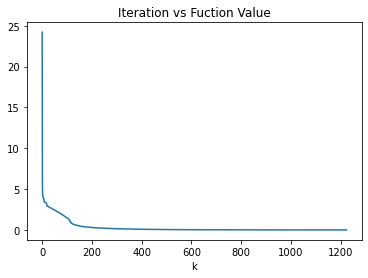
\includegraphics[width=0.8\linewidth]{graficas/rosembrock_backtracking_2f}
	\\
	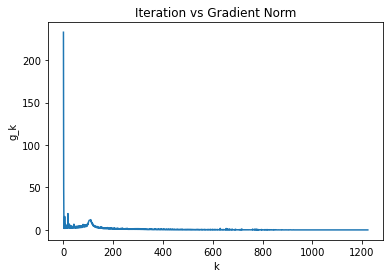
\includegraphics[width=0.8\linewidth]{graficas/rosembrock_backtracking_2g}
	\\
	Gráficas para Bisección
	\\
	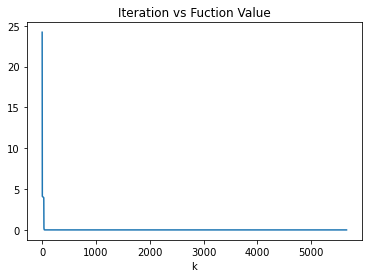
\includegraphics[width=0.8\linewidth]{graficas/rosembrock_bisection_2f}
	\\
	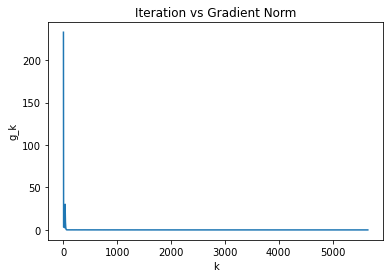
\includegraphics[width=0.8\linewidth]{graficas/rosembrock_bisection_2g}
\end{center}

Para $ n = 100 $ con $ x_0 = [-1.2, 1, \dots, -1.2, 1] $ y parámetros
\begin{center}
	\begin{tabular}{cc}
		\hline
		Parámetro & Valor \\
		\hline
		$\alpha $ & 0.1 \\
		$ \rho $  & 0.5 \\
		$ c_1 $ & $ 10^{-4} $ \\
		$ c_2 $  & $ 0.9 $ \\
		\hline
	\end{tabular}
\end{center}
se obtuvo
\begin{center}
	\begin{tabular}{cc}
		\hline
		Algoritmo & Iteraciones \\
		\hline
		BackTracking & 800 \\
		Bisección  & 617 \\
		\hline
	\end{tabular}
	\\
	Gráficas para Backtracking
	\\
	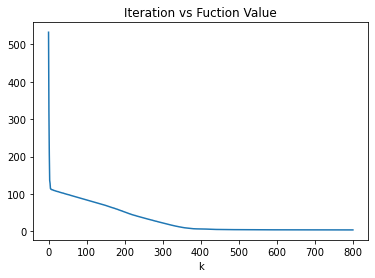
\includegraphics[width=0.8\linewidth]{graficas/rosembrock_backtracking_100f}
	\\
	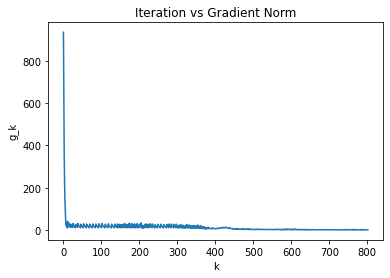
\includegraphics[width=0.8\linewidth]{graficas/rosembrock_backtracking_100g}
	\\
	Gráficas para Bisección
	\\
	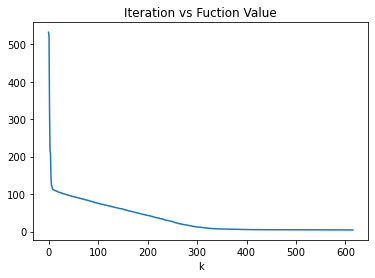
\includegraphics[width=0.8\linewidth]{graficas/rosembrock_bisection_100f}
	\\
	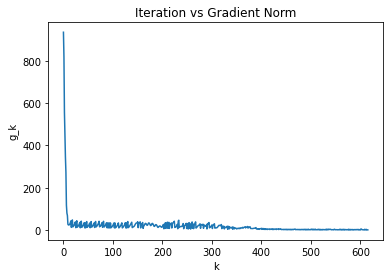
\includegraphics[width=0.8\linewidth]{graficas/rosembrock_bisection_100g}
\end{center}
\textbf{Observación.} Sin embargo no fue posible que el mínimo correspondiera al punto $ [1,\dots, 1] $. Para ello se introduce un punto inicial aleatorio.

\subsubsection{Puntos iniciales aleatorios}
Se generaron puntos iniciales usando la distribución normal de media cero y desviación 1. Se repitió el experimento $ 50 $ veces
\\
Para $ n = 2 $ se obtuvo
\begin{center}
	\begin{tabular}{ccc}
		\hline
		Algoritmo & Tiempo Promedio & Promedio Iter \\
		\hline
		BackTracking & 0.1238 & 906.14 \\
		Bisección     & 0.8856 & 1915.48\\
		\hline
	\end{tabular}
\end{center}
Para $ n = 100 $ se repitió un total de $ 5 $  veces. Se observó que al generar un punto inicial aleatorio sí se llegó al máximo global $[1,1,\dots, 1]$
\begin{center}
	\begin{tabular}{ccc}
		\hline
		Algoritmo & Tiempo Promedio & Promedio Iter \\
		\hline
		BackTracking & 25.69 & 5154.0 \\
		Bisección     & 54.28 & 2344.2\\
		\hline
	\end{tabular}
\end{center}
\subsection{Función de Wood}
Para $ x_0 = [-3.0, -1-0, -3.0, -1.0] $ y parámetros
\begin{center}
	\begin{tabular}{cc}
		\hline
		Parámetro & Valor \\
		\hline
		$\alpha $ & 0.9 \\
		$ \rho $  & 0.5 \\
		$ c_1 $ & $ 10^{-4} $ \\
		$ c_2 $  & $ 0.9 $ \\
		\hline
	\end{tabular}
\end{center}
se obtuvo
\begin{center}
	\begin{tabular}{cc}
		\hline
		Algoritmo & Iteraciones \\
		\hline
		BackTracking & 2871 \\
		Bisección  & 7527 \\
		\hline
	\end{tabular}
	\\
	Gráficas para Backtracking
	\\
	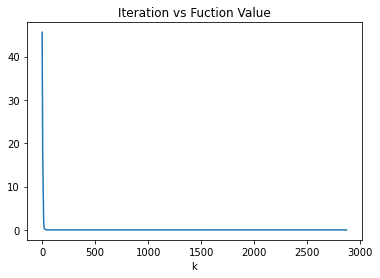
\includegraphics[width=0.8\linewidth]{graficas/wood_backtracking_f}
	\\
	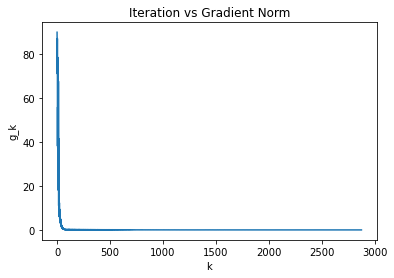
\includegraphics[width=0.8\linewidth]{graficas/wood_backtracking_g}
	\\
	Gráficas para Bisección
	\\
	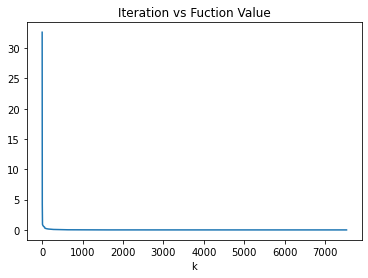
\includegraphics[width=0.8\linewidth]{graficas/wood_bisection_f}
	\\
	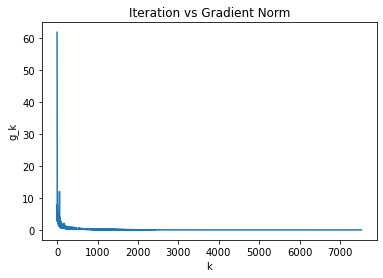
\includegraphics[width=0.8\linewidth]{graficas/wood_bisection_g}
\end{center}
\subsubsection{Puntos iniciales aleatorios}
Se generaron puntos iniciales usando la distribución normal de media cero y desviación uno. Se repitió el experimento $ 50 $ veces y se obtuvo
\begin{center}
	\begin{tabular}{ccc}
		\hline
		Algoritmo & Tiempo Promedio & Promedio Iter \\
		\hline
		BackTracking & 0.061 & 311.66 \\
		Bisección    & 0.184 & 232.94 \\
		\hline
	\end{tabular}
\end{center}

\subsection{Función $ f_3 $}
Se generó un vector inicial $ x_0 $ y $ eta $ de tamaño $ n = 128 $ de manera aleatoria siguientdo una distribución $ \mathcal{N}(0, \sigma) $. Por motivos de practicidad se fijó $ \sigma = 1 $.
\\
Para $ \lambda = 1 $ y los parámetros
\begin{center}
	\begin{tabular}{cc}
		\hline
		Parámetro & Valor \\
		\hline
		$\alpha $ & 0.2 \\
		$ \rho $  & 0.5 \\
		$ c_1 $ & $ 10^{-4} $ \\
		$ c_2 $  & $ 0.9 $ \\
		\hline
	\end{tabular}
\end{center}
se obtuvo
\begin{center}
	\begin{tabular}{cc}
		\hline
		Algoritmo & Iteraciones \\
		\hline
		BackTracking & 2441 \\
		Bisección    & 8 \\
		\hline
	\end{tabular}
	\\
	Gráficas para Backtracking
	\\
	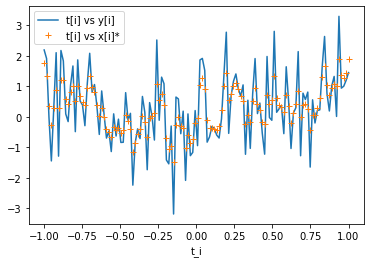
\includegraphics[width=0.8\linewidth]{graficas/f3_backtracking_lambda1}
	\\
	Gráficas para Bisección
	\\
	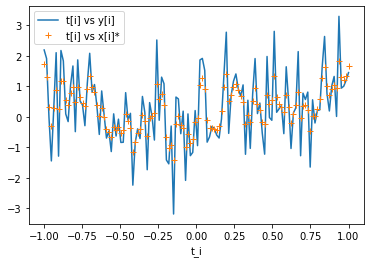
\includegraphics[width=0.8\linewidth]{graficas/f3_bisection_lambda1}
\end{center}

Para $ \lambda = 10 $ y los parámetros
\begin{center}
	\begin{tabular}{cc}
		\hline
		Parámetro & Valor \\
		\hline
		$\alpha $ & 0.2 \\
		$ \rho $  & 0.5 \\
		$ c_1 $ & $ 10^{-4} $ \\
		$ c_2 $  & $ 0.9 $ \\
		\hline
	\end{tabular}
\end{center}
se obtuvo
\begin{center}
	\begin{tabular}{cc}
		\hline
		Algoritmo & Iteraciones \\
		\hline
		BackTracking & 19 \\
		Bisección    & 17 \\
		\hline
	\end{tabular}
	\\
	Gráficas para Backtracking
	\\
	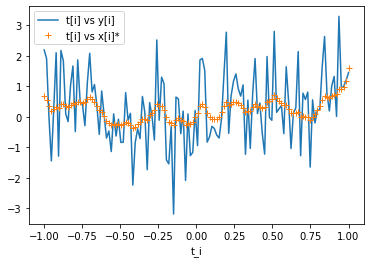
\includegraphics[width=0.8\linewidth]{graficas/f3_backtracking_lambda10}
	\\
	Gráficas para Bisección
	\\
	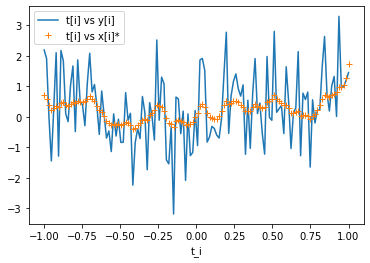
\includegraphics[width=0.8\linewidth]{graficas/f3_bisection_lambda10}
\end{center}

Para $ \lambda = 1000 $ y los parámetros
\begin{center}
	\begin{tabular}{cc}
		\hline
		Parámetro & Valor \\
		\hline
		$\alpha $ & 0.2 \\
		$ \rho $  & 0.5 \\
		$ c_1 $ & $ 10^{-4} $ \\
		$ c_2 $  & $ 0.9 $ \\
		\hline
	\end{tabular}
\end{center}
se obtuvo
\begin{center}
	\begin{tabular}{cc}
		\hline
		Algoritmo & Iteraciones \\
		\hline
		BackTracking & 13 \\
		Bisección    & 18 \\
		\hline
	\end{tabular}
	\\
	Gráficas para Backtracking
	\\
	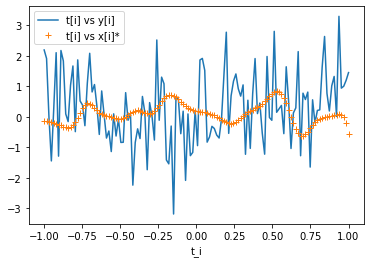
\includegraphics[width=0.8\linewidth]{graficas/f3_backtracking_lambda1000}
	\\
	Gráficas para Bisección
	\\
	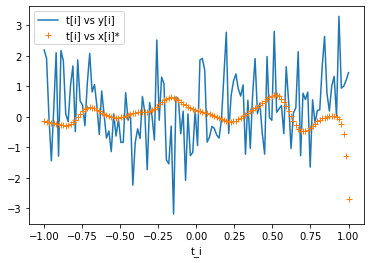
\includegraphics[width=0.8\linewidth]{graficas/f3_bisection_lambda1000}
\end{center}





\subsubsection{Puntos iniciales aleatorios}
Se generaron puntos iniciales usando la distribución normal de media cero y desviación uno. Se repitió el experimento $ 20 $ veces y se usó $ \lambda = 10 $. Los resultados fueron
\begin{center}
	\begin{tabular}{ccc}
		\hline
		Algoritmo & Tiempo Promedio & Promedio Iter \\
		\hline
		BackTracking & 0.1075 & 128 \\
		Bisección    & 0.4285 & 128 \\
		\hline
	\end{tabular}
\end{center}
\section{Conclusiones}
	\subsection{Rosembrock}
	Para esta función se observa un mejor desempeño en el algoritmo de backtracking que en el de bisección (con respecto al número de iteraciones). De hecho, en las gráficas mostradas el decrecimiento del valor $ f(x_k) $ y $ g(x_k) $ es más suave para bactracking que para bisección.
	\\
	Además, para $ n = 100 $ y con el punto inicial sugerido, no fue posible llegar al mínimo $ [1, 1, \dots, 1]^T $. Pero cuando se utilizó un vector inicial aleatorio, el método sí fue capaz de llegar al mínimo de unos.
	\\
	Para la experimentación aleatoria se observa, de nuevo, un mejor desempeño en el método de backtracking que en el de bisección.
	
	\subsection{Wood}
	En esta función, un cambio sutil en los parámetros, hacía llegar el punto inicial sugerido a otros mínimos locales. Se observó, de nuevo, que backtracking convergió en un menor número de iteraciones y en las gráficas se observa un decrecimiento tanto de $ f(x_k) $ como de $ ||g(x_k) || $ rápido pero para el algoritmo de bisección se ve menor suavidad.
	
	\subsection{Función $ f_3 $}
	En esta función, el valor $ \eta $ está causando ruido en la ''parábola´´ descrita por $ f(x) $. Observemos que para $ \lambda = 1 $ el error de aproximación es menor que para $ \lambda = 10, 1000 $. En general, cuando se fijó $ x_0 $, la convergencia se logró en menos de $ 20 $ iteraciones. 

\end{document}